\chapter{Literature Review}

\section{Introduction}
This chapter covers literature review on algorithm selection and reinforcement learning. The discussion focuses on background and methods surrounding these topics. The last section discusses the reinforcement learning approach to algorithm selection.

\section{Algorithm Selection}
The algorithm selection (AS) problem describes how a set of problems can be mapped to a set of algorithms such that the least amount of computing resources are spent to solve the whole set of problems \citep{rice1976algorithm}. A model of the AS problem is depicted in Figure \ref{fig:asmodel}.

\begin{figure}[H]
	\centering
	 \scalebox{.7}{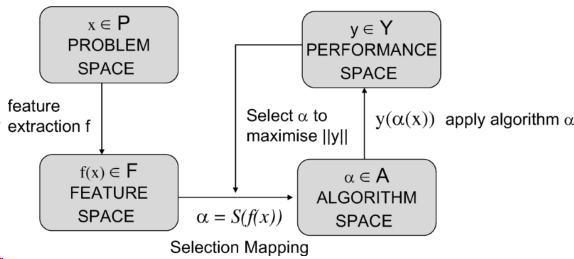
\includegraphics{./img/as_model.png}}
	\caption{Model of the AS problem}
	\label{fig:asmodel}
\end{figure}

An AS model is composed of four components: \textit{problems, features, algorithms,} and \textit{performance}.

\begin{enumerate}
	\item Problem space ($\mathbf{P}$) \\
	The set of problem instances. Instances are often grouped into \textit{problem classes}, which categorize their level of difficulty. The number of problems are usually vast and diverse.
	\item Feature space ($\mathbf{F}$) \\
	The set of features describing the problem instances. Specifically, features define the measurable characteristics of problems, which provides an indication on the difficulty of problems.
	\item Algorithm space ($\mathbf{A}$) \\
	The set of algorithms used to solving the problem instances. A large number of algorithms could be possibly used, but practically only a handful is considered.
	\item Performance space ($\mathbf{Y}$) \\
	The set of metrics that defines how algorithm performance is measured.
\end{enumerate}

Formally stating the AS problem, 

\fbox{
\begin{minipage}{\dimexpr\textwidth-1cm}
\textit{Given problem instance $x \in \mathbf{P}$ with features $f(x) \in \mathbf{F}$ , find a selection mapping $\alpha = S(f(x))$ in algorithm space $\mathbf{A}$, where the selected algorithm $\alpha \in \mathbf{A}$ provides the maximum performance $y(\alpha(x)) \in \mathbf{Y}$ in solving the problem instance $x \in \mathbf{P}$.}
\end{minipage}
}

\subsection{Motivation}
AS is based on the observation that there is no single algorithm that can optimally solve all kinds of problems. The \textit{No Free Lunch} (NFL) theorems assert that on a set of problems with varying degrees of difficulty, all algorithms perform the same on average \citep{wolpert1997no}. This implies that if an algorithm executes well on one class of problems, it pays off for decreased performance on other classes. NFL theorems have been demonstrated on problems such as search \citep{wolpert1995no}, cross validation \citep{goutte1997note}, multiobjective optimization \citep{corne2003no}, and sparse approximation \citep{xu2012sparse}.

\begin{figure}[H]
	\centering
	\scalebox{.6}{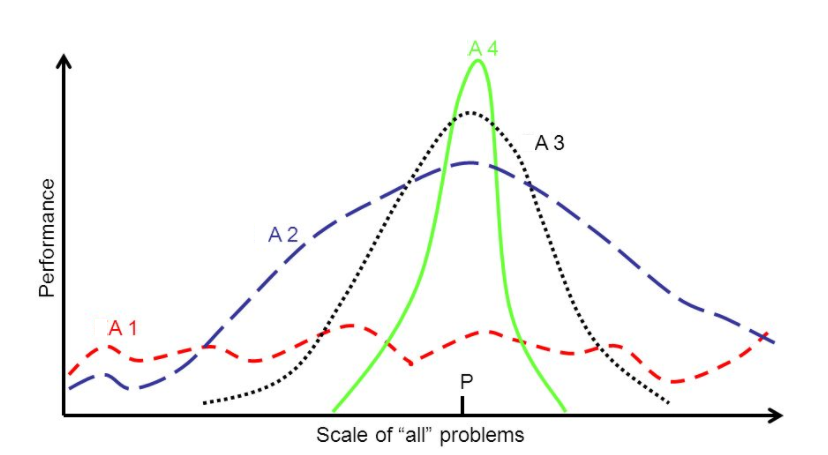
\includegraphics{./img/algo_perf_dist.png}}
	\caption{Typical distribution of algorithms with respect to performance}
	\label{fig:algoperfdist}
\end{figure}

The NFL theorems suggest to shift the focus of solving problems to AS. Learning the problem characteristics can help in deciding which algorithm is most suitable in solving a problem. Also, a set of algorithms with complementary strengths is desirable. A collection of algorithms used for solving a set of problems is called an \textit{algorithm portfolio}.

\subsection{Algorithm Portfolios}
Algorithm portfolios combine multiple algorithms with complementary strengths in order to solve problems more efficiently. This is inspired by \textit{investment portfolios} concept in Economics where maximizing a utility with associated risks is handled by mixing strategies with desired risk and performance \citep{huberman1997economics}.

\begin{figure}[H]      
	\scalebox{.7}{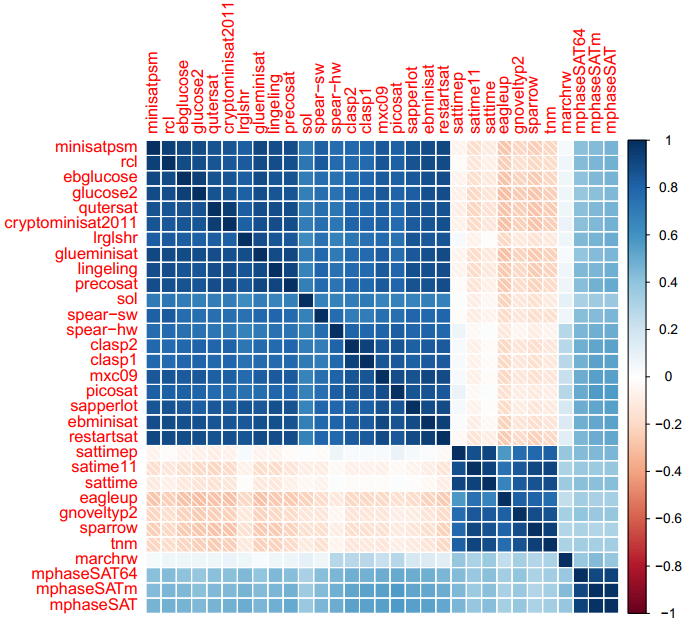
\includegraphics{./img/sat_correl.png}}
	\caption[Correlation matrix of SAT solvers]{Correlation matrix of SAT solvers. Solvers with less correlation have more complementary performance. Red and blue boxes indicate negative and positive correlation respectively; shading represents the correlation strength \citep{bischl2016aslib}}
	\label{fig:satcorrel}
\end{figure}

Using algorithm portfolios have been proven effective on solving hard combinatorial problems \citep{gomes2001algorithm}. Gomes and Selman concluded that algorithm portfolios can obtain superior performance by exploiting the variance in behavior among algorithms. One AS technique that takes advantage of this is called \textit{presolving}. Presolving makes use of \textit{presolvers}, which basically are algorithms that execute quickly and can solve a large number of problems \citep{xu2008satzilla}. Presolvers tend to eliminate the easier problems so AS can focus on solving the much harder problems.

\subsection{Problem Domain}
AS can be best applied on combinatorial search and optimization problems. One example is the Boolean satisfiability (SAT) problem, a classic NP-complete problem of finding assignments of variables to a Boolean formula such that it evaluates to TRUE. Successful AS implementations include SATzilla \citep{xu2008satzilla}, SATenstein \citep{khudabukhsh2009satenstein}, and Hydra \citep{xu2010hydra}. Efficient SAT solvers benefit applications such as IC design, computer-aided design and manufacturing, and automated theorem proving.

\begin{figure}[H]
	\centering
	\scalebox{.9}{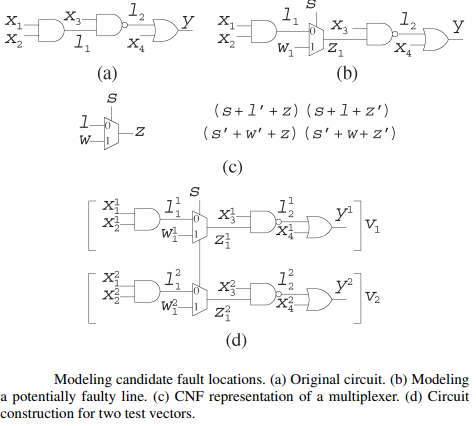
\includegraphics{./img/logic_circuits.png}}
	\caption[Fault-diagnosis of very-large-scale-integration (VLSI) circuits modelled as a SAT problem]{Fault-diagnosis of very-large-scale-integration (VLSI) circuits modelled as a SAT problem. \citep{smith2005fault}}
	\label{fig:logiccircuits}
\end{figure}

Travelling salesman problem (TSP), a famous example of an \textit{NP}-hard problem, also benefits from AS. Given a list of points and the associated costs between pairs of points, the goal of TSP is to find a path with minimum total cost between two selected points. Points can represent destinations or, in a more abstract sense, nodes in a graph. Costs can refer to distance or any measure that represents the weight of relationship between a pair of nodes in a graph. An algorithm portfolio of inexact TSP solvers showed significant performance improvements after AS \citep{kotthoff2015improving}. The travelling thief problem \citep{bonyadi2013travelling}, a combination of TSP and knapsack problem \citep{kellerer2004introduction}, has also been tackled using AS techniques, resulting in substantial improvements over single solvers \citep{wagner2018case}. 

\begin{figure}[H]
	\centering
	\scalebox{.6}{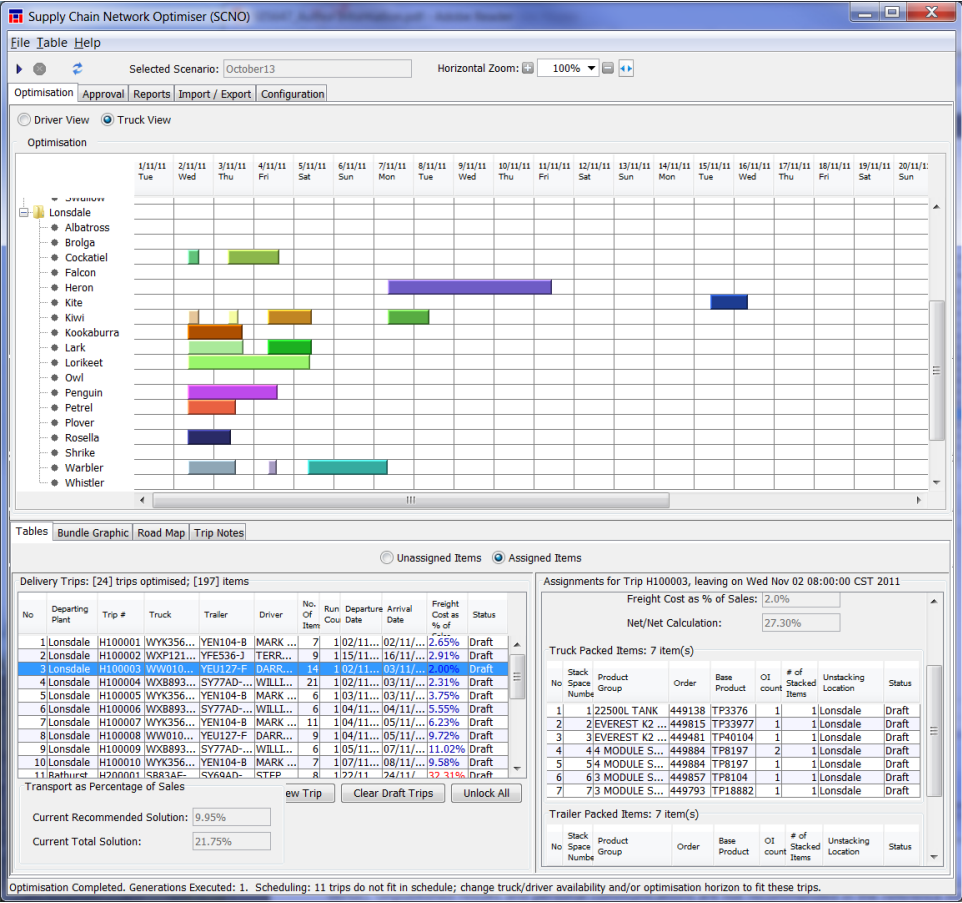
\includegraphics{./img/water_tank.png}}
	\caption[Water tank delivery schedule generated by an optimizer software]{Water tank delivery schedule generated by an optimizer software. This demonstrates the real-world application of the solution to travelling thief problem. \citep{stolk2013combining}}
	\label{fig:watertank}
\end{figure}

In this study, AS is applied on solving subgraph isomorphism problems. This is an \textit{NP}-complete problem whereby a smaller graph is located in a larger graph. As the number of graph nodes increases, the amount of effort expended in searching for subgraph isomorphisms exponentially increases. Using AS to search for subgraph isomorphisms have demonstrated significant performance improvements over standalone algorithms (\citet{battiti2007algorithm}; \citet{kotthoff2016portfolios}). Subgraph isomorphism problems manifest in applications that use graphs to model problems. A few examples include chemistry, software engineering, and biocomputing.

\begin{figure}[H]
	\centering
	\scalebox{.7}{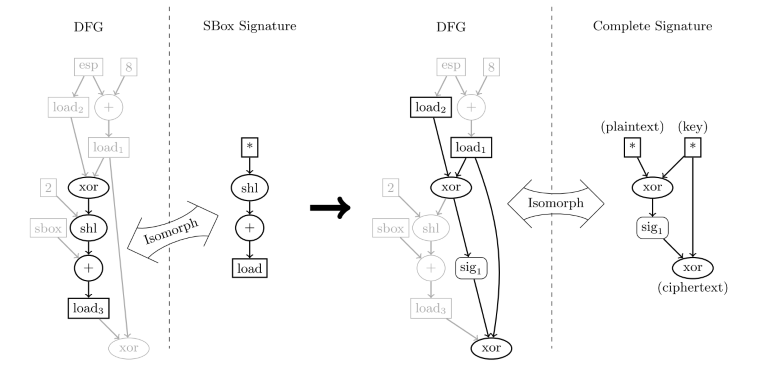
\includegraphics{./img/flowchart.png}}
	\caption[Identifying malware in executable files through recognition of cryptographic algorithm patterns]{Identifying malware in executable files through recognition of cryptographic algorithm patterns. Searching for a cryptographic signature (pattern graph) from the program's data flow graph (DFG) is a subgraph isomorphism problem. \citep{lestringant2015automated}}
	\label{fig:flowchart}
\end{figure}

Combining the strengths of several algorithms through AS can lead to more efficient solutions to hard combinatorial problems. In retrospect, AS does not entirely discourage the formulation of new algorithms. Research in AS seeks not only to improve problem solving performance, but also to learn more about the nature of problems and the behaviors of algorithms used. It can also provide valuable insights in creating new algorithms or improving upon existing ones. Studies on new algorithms are just as important as AS research, since the effectiveness of AS still relies on how well individual algorithms perform.

\section{Algorithm Selection Techniques}
A comprehensive review of AS techniques can be referred from Smith-Miles \citep{smith2009cross} and Kotthoff \citep{kotthoff2016algorithm}. Typically, the following are considered when creating a new AS technique:

\begin{enumerate}
	\item How can algorithm portfolios be constructed? (e.g. static portfolios vs. dynamic portfolios)
	\item What algorithms to select and when? (e.g. single algorithm per problem vs. multiple algorithms with scheduling)
	\item How to select algorithms? (modelling algorithm performance with respect to problems)
\end{enumerate}

This study is limited to the use of a static portfolio and the selection of one algorithm per problem instance. This section mainly discusses techniques in (3). 

On most approaches, machine learning is used to discover the relationship between algorithms and problems.  This often includes a training phase, where algorithms are executed on a subset of problems to evaluate their performance. The general approach to AS \citep{bischl2016aslib} is depicted in Figure \ref{fig:asworkflow}.

\begin{figure}[H]
	\centering
	\scalebox{.6}{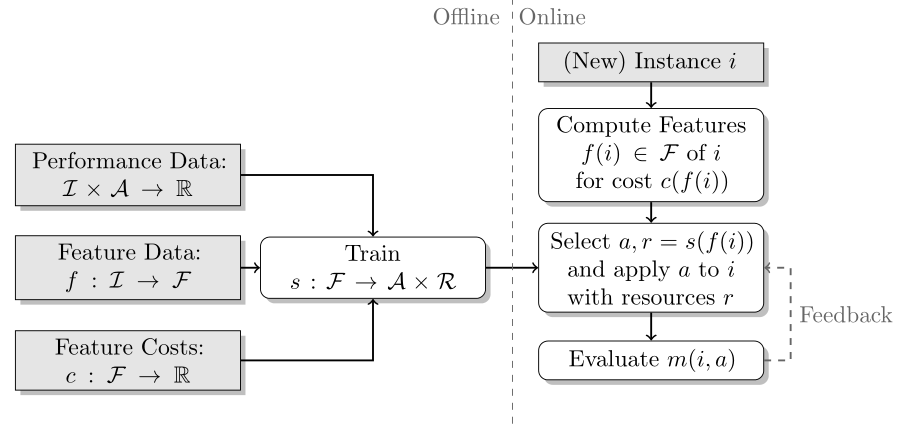
\includegraphics{./img/as_workflow.png}}
	\caption[AS workflow]{AS workflow.}
	\label{fig:asworkflow}
\end{figure}

\begin{enumerate}
	\item For each problem instance \textit{i}, a vector of instance features $f(i) \in \mathbf{F}$ is computed. 
	\item A machine learning technique \textit{s} selects an algorithm $a \in \mathbf{A}$ based on the feature vector from Step 1.
	\item The selected algorithm \textit{a} is applied to problem instance \textit{i}.
	\item Performance measure \textit{m} is evaluated, taking into account feature computation costs and the performance of the selected algorithm.
\end{enumerate}

Choosing a machine learning technique is often based from the nature of the problem to be solved. For instance, a classification model is viable for simple problem-algorithm mappings. Each problem can be labeled with the best-performing algorithm, then the classifier is trained to recognize problems and their corresponding optimal algorithms. One classifier implementation used a decision tree that assigned slower or faster algorithms to constraint satisfaction problems \citep{gent2010learning}. 

\begin{figure}[H]
	\centering
	\scalebox{.7}{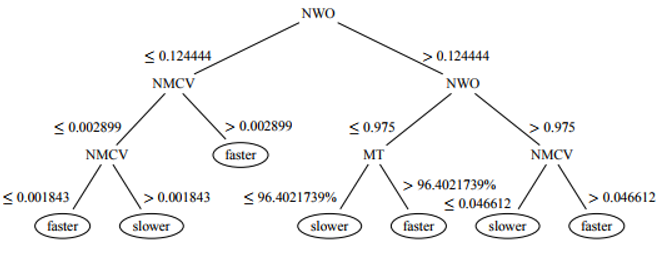
\includegraphics{./img/decision_tree.png}}
	\caption[Decision tree classifier built using C4.5 algorithm]{Decision tree classifier built using C4.5 algorithm.Nodes represent attribute rules the guide the decision of choosing a ‘slower’ or a ‘faster’ algorithm for a problem. \citep{gent2010learning}}
	\label{fig:decisiontree}
\end{figure}

Alternatively, algorithm performance can be predicted using regression models. Training is slower since it is done for each algorithm per problem instance, as opposed to classification models where training iterates only for each problem instance. The advantage is that models are learned per individual algorithm instead of the whole algorithm portfolio, as with the case for classification models. SATzilla, a SAT solver that dominated SAT competitions, used ridge regression to learn an AS model of SAT problems \citep{xu2008satzilla}. For subgraph isomorphism problems, pairwise random forest regression stands as the current best approach \citet{kotthoff2016portfolios}. 

\begin{figure}[H]
	\centering
	\scalebox{.7}{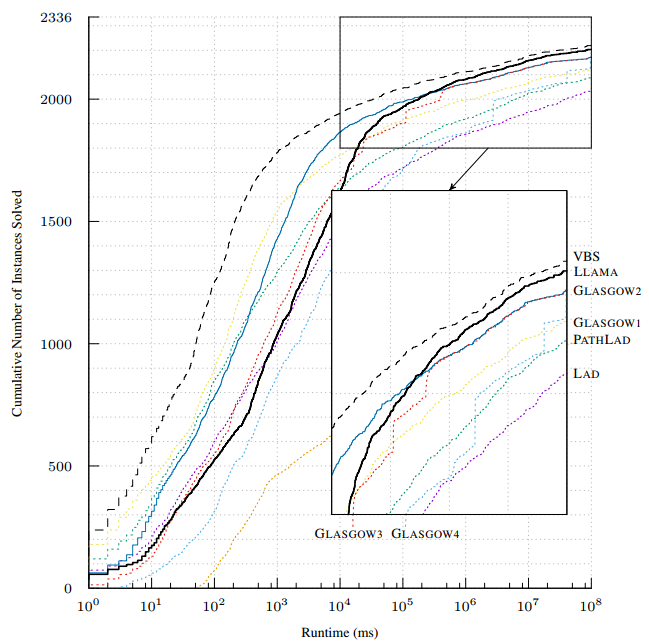
\includegraphics{./img/subgraph_isomorphism.png}}
	\caption[Performance comparison of subgraph isomorphism algorithms]{ Performance comparison of subgraph isomorphism algorithms. \textit{LLAMA} is the AS model trained using pairwise random forest regression. Its performance comes near the virtual best solver (VBS)—the upper-bound of what an AS model can achieve in an algorithm portfolio. \citep{kotthoff2016portfolios}}
	\label{fig:subgraphisomorphism}
\end{figure}

Another approach is to group problem instances into clusters and assign the cost-optimal solver for each cluster. This approach is useful when there is minimal knowledge about the problem. One example did not rely on problem features to do AS; instead a model of algorithm performance behavior is learned and then used to identify clusters of similar problems \citep{silverthorn2010latent}. The AS model gathered roughly competitive results after comparing against SATzilla.

\begin{table}[H]
	\centering
	\begin{tabular}{llll}
		\hline
		\multicolumn{1}{c}{\multirow{2}{*}{\textbf{Method}}} & \multicolumn{3}{c}{\textbf{SAT Instances Solved}} \\ \cline{2-4} 
		\multicolumn{1}{c}{} & \multicolumn{1}{c}{random} & \multicolumn{1}{c}{crafted} & \multicolumn{1}{c}{indust.} \\ \hline
		Best Single & 320.8 (3.7) & 122.6 (3.8) & \textbf{153.5 (3.2)} \\
		Random & 261.6 (4.8) & 89.3 (3.5) & 54.5 (3.4) \\
		SATzilla & 407.5 (3.1) & 125.6 (3.3) & 137.6 (3.3) \\
		Soft + Mult. & 319.3 (8.2) & 116.9 (4.9) & 136.2 (4.3) \\
		Soft + DCM & 342.2 (8.2) & 118.2 (4.3) & 138.1 (5.0) \\
		Hard + Mult. & 340.3 (45.7) & 104.8 (9.7) & 129.4 (8.0) \\
		Hard + DCM & \textbf{424.2 (12.9)} & \textbf{129.4 (6.5)} & 146.0 (5.6) \\ \hline
	\end{tabular}
	\caption[Comparison of the number of SAT problems solved between SATzilla vs. latent class clustering models]{Comparison of the number of SAT problems solved between SATzilla vs. latent class clustering models. The last four methods in the table correspond to different latent class methods used. \citep{silverthorn2010latent}}
	\label{tbl:satzilla}
\end{table}

Several machine-learning approaches to AS exist, such as hybrid regression-classification models \citep{kotthoff2012hybrid}, ensembles \citep{kotthoff2010ensemble}, and reinforcement learning \citep{lagoudakis2000algorithm}. 

\section{Reinforcement Learning Approach to Algorithm Selection}
Training AS models typically use classification or regression methods (or a hybrid of these two) due to the complete availability of information on problems and algorithm performance. Reinforcement learning (RL) techniques are typically used when dynamic (a.k.a. online learning) AS is necessary, where the AS model continuously adapts and learns as it solves more problems. One example is an AS model trained using a modified Q-learning algorithm \citep{lagoudakis2000algorithm}. The model continuously learns to select algorithms that minimize the overall time in solving all problems. A more sophisticated application used a multi-armed bandit approach to AS where the model progressively learns how to efficiently schedule and distribute problem solving across multiple CPUs \citep{gagliolo2009towards}.

RL encompasses computational methods in learning from interactions with the environment to achieve long term goals \citep{sutton1998reinforcement}. An \textit{agent} perceives the \textit{state} of its \textit{environment} and receives \textit{feedback} (instantly or time-delayed) for every \textit{action} it takes. Feedback can be understood as rewards in which the agent seek to maximize over time. Learning is driven by the interaction between agent and environment: the environment provides stimulus to the agent, and then the agent makes decisions on how to respond. In RL terms this is called \textit{policy} – a set of rules that guides agent behavior.

Figure \ref{fig:rlmodel} summarizes the main idea behind RL. The RL model can be framed in the context of AS by mapping its elements to the model of AS problem (Figure 2.1). This is shown in Figure \ref{fig:rlasmodel}.

\begin{figure}[H]
	\centering
	\scalebox{.5}{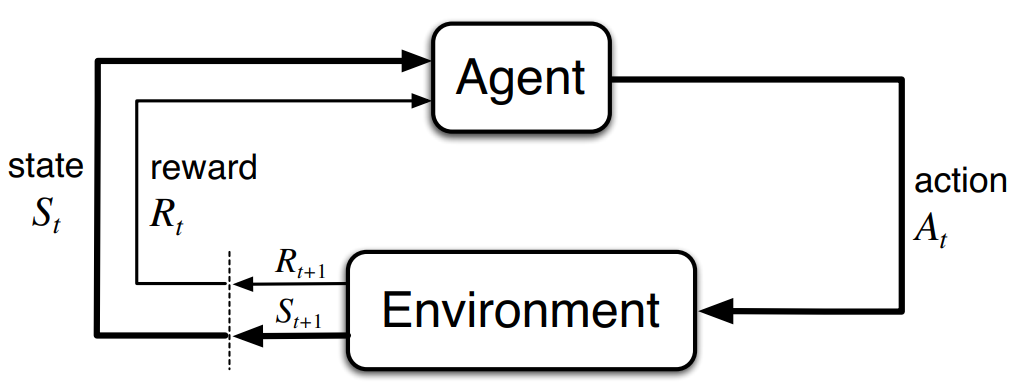
\includegraphics{./img/rl_model.png}}
	\caption{Reinforcement learning model}
	\label{fig:rlmodel}
\end{figure}

\begin{figure}[H]
	\centering
	\scalebox{.85}{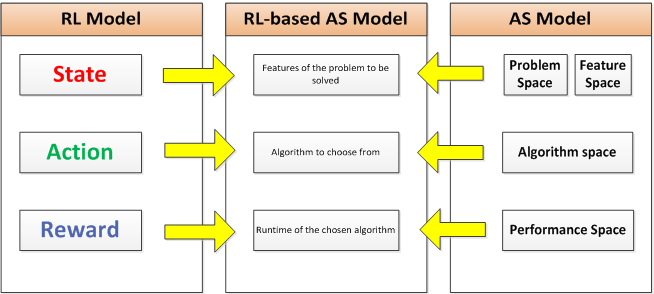
\includegraphics{./img/rlas_model.png}}
	\caption{Reinforcement learning-based algorithm selection model}
	\label{fig:rlasmodel}
\end{figure}

\subsection{Policy Gradient Methods}

The agent's \textit{policy} is a function that outputs an action based from the input environment state. It can be learned by applying some performance measure and monitoring how it changes with respect to the environment state. \textit{Policy gradient} methods represent a class of techniques under RL that learns a policy through change in performance measure. These methods seek to maximize long term rewards by optimizing performance.

\begin{equation}
\mathbf{\theta_{t+1}} = \mathbf{\theta_t} + \alpha \nabla J(\theta_t)
\label{eq:pgrad}
\end{equation}

This study uses REINFORCE algorithm \citep{williams1992simple} to train an AS model. The acronym describes the policy parameter update equation used in its algorithm: \textbf{RE}ward \textbf{IN}crement \textit{equals} \textbf{N}onnegative \textbf{F}actor \textit{plus} \textbf{O}ffset \textbf{R}einforcement \textit{plus} \textbf{C}haracteristic \textbf{E}ligibility. 

\begin{equation}
\mathbf{\theta_{t+1}} = \mathbf{\theta_t} + \alpha G_t \frac{\nabla_\theta\pi(A_t|S_t, \theta_t)}{\pi(A_t|S_t, \theta_t)}
\label{eq:reinforce}
\end{equation}

The intuition behind Equation \ref{eq:reinforce} is as follows: each increment is proportional to the product of a reward $G_t$ and a vector, the gradient of the probability of taking the action actually taken, $\nabla_\theta\pi(A_t|S_t, \theta_t)$, divided by the probability of taking that action $\pi(A_t|S_t, \theta_t)$. The vector is the direction in parameter space that most increases the probability of repeating the action $A_t$ on future visits to state $S_t$. The update increases the parameter vector in this direction proportional to the reward, and inversely proportional to the action probability. The former makes sense because it causes the parameter to move most in the directions that favor actions that yield the highest reward. The latter makes sense because otherwise actions that are selected frequently are at an advantage (the updates will be more often in their direction) and might win out even if they do not yield the highest return. \citep{sutton1998reinforcement}. 